\documentclass[]{auvsi_doc}
\setkeys{auvsi_doc.cls}{
	AUVSITitle={2019 AUVSI Competition Summary},
	AUVSIRevision=0.0,
	AUVSIDescription={Created},
	AUVSIAuthor={Derek Knowles},
	AUVSIChecker={[Checker]},
	AUVSILogoPath={./figs/logo.pdf},
	AUVSIDocID={AF-012}
}

% include extra packages, if needed
\usepackage{makecell}
\usepackage{longtable}
\usepackage{hyperref}
\usepackage{booktabs}

\usepackage{pdfpages}
% Remove Heading Numbers
\setcounter{secnumdepth}{0}
\providecommand{\tightlist}{%
  \setlength{\itemsep}{0pt}\setlength{\parskip}{0pt}}

\begin{document}
\begin{AUVSITitlePage}
\begin{artifacttable}
	\entry{PS-001, 0.1, 06-17-2019, Created, Kameron Eves, Jacob Willis}
	\entry{PS-001, 1.0, 07-29-2019, Converted to Latex, Jacob Willis, Jake Johnson}
\end{artifacttable}
\end{AUVSITitlePage}
% document contents
\section{Introduction}
This document summarizes the results from the AUVSI Competition, held June 12th - 15th, 2019.

\section{Pre-Competition}
We got lucky and drew got to choose our flight time second. (there is some speculation that our high paper and video scores helped us get to choose our flight time first).
We choose one of the last times on Saturday morning, so we could hammer out some bugs.

We spent basically all-day Wednesday, Thursday, and Friday debugging, tuning gains, flight testing, and repeating. We had a minor crash on Friday when we drained the battery in flight and ended up in a tree. Luckily it was in the tree and not on the ground because it was suspended right over the biggest puddle ever. Blessedly, there was no damage. Also, of note, we removed the filleted paths from the path manager because it was causing us to fly away into the distance without making turns. This worked, but we didn’t test it for the first time until the competition.

\section{Competition}
We were surprised on Saturday with how quickly we got to the flight line (we flew basically as soon as we got there), so things were a bit rushed. The weather was windy, but overall favorable. The mission proceeded as follows:
\begin{itemize}
	\item    Andrew gave a boss briefing, nameing each team member and describing their role.
	\item    Manual takeoff. An autonomous takeoff should work, but we didn’t want to try it for the first time in the competition and didn't want to risk testing it just a day or two before the competition.
	\item    We began autonomous flight immediately after take off and loitered for 3 minutes. We wanted to ensure we got the full autonomous flight points because we weren’t 100 percent confident in the path manager. In hindsight this was a mistake, the path manager worked fine, and we ran out of time in the end.
	\item    The aircraft planned, flew, and hit the waypoints beautifully and fully autonomously. However, we did not notice until we received our score that we forgot to change one parameter (the location of the origin used by the interop client). This meant that for our entire flight we reported our location to interop as if we were in the park where we spent the week testing and not at the actual competition field. Changing this parameter was on the checklist but got skipped in our rush. So, we got no points for hitting the waypoints. On the plus side, because we were reporting our location incorrectly by several miles, we also didn’t hit any obstacles (although this benefit was negligible).
	\item    We then planned and attempted an autonomous UGV drop. We flew the path successfully but the command to actually drop was not sent autonomously (there's probably a bug in the payload drop code, this was one of the first autonomous drop attempts). So, we took over RC, flew the path manually, and sent the drop command manually. This worked; however, we did not have enough accuracy to hit the target this way. So, we got no points from this portion of the competition.
	\item    We then entered an autonomous loiter while we planned a search path for the vision team. This in hindsight was also a bad idea. The drop location was right next to a boundary and the tents, so we flew out of bounds and over the tents. They called this an “Unsafe Out of Bounds” and we received a huge penalty for it (Equivalent to all our autonomous flight points).
	\item    We then attempted to fly the search path, while flying the search path we realized it was going to take too long to fly there autonomously and so Kameron manually took over for a third time and flew over as much of the search area as he could before we ran out of time. We successfully identified 4 targets manually, and one target autonomously. We actually were the only team to successfully identify a target autonomously. We received the Cyber Award for it.
	\item    At that point we didn’t have time to continue searching for targets and returned for a manual landing. (An autonomous landing would have given us no additional points while also risking a fourth manual takeover.)
	\item    We exited the airfield with seconds to spare.
\end{itemize}

In the end we received a score of 25th for the flight, 3rd for the Mission Readiness Review and 5th for the Journal, resulting in 17th overall. 
All in all, we’re proud of the performance and don’t feel like our score represented our actual performance. Because our paper and flight readiness review were so good, and because we were the only team to autonomously identify a target, we received \$1,750 in prize money. (More than last year.)


\section{Appendix: Judges Feedback}
Included here is the feedback we received from the Judges.
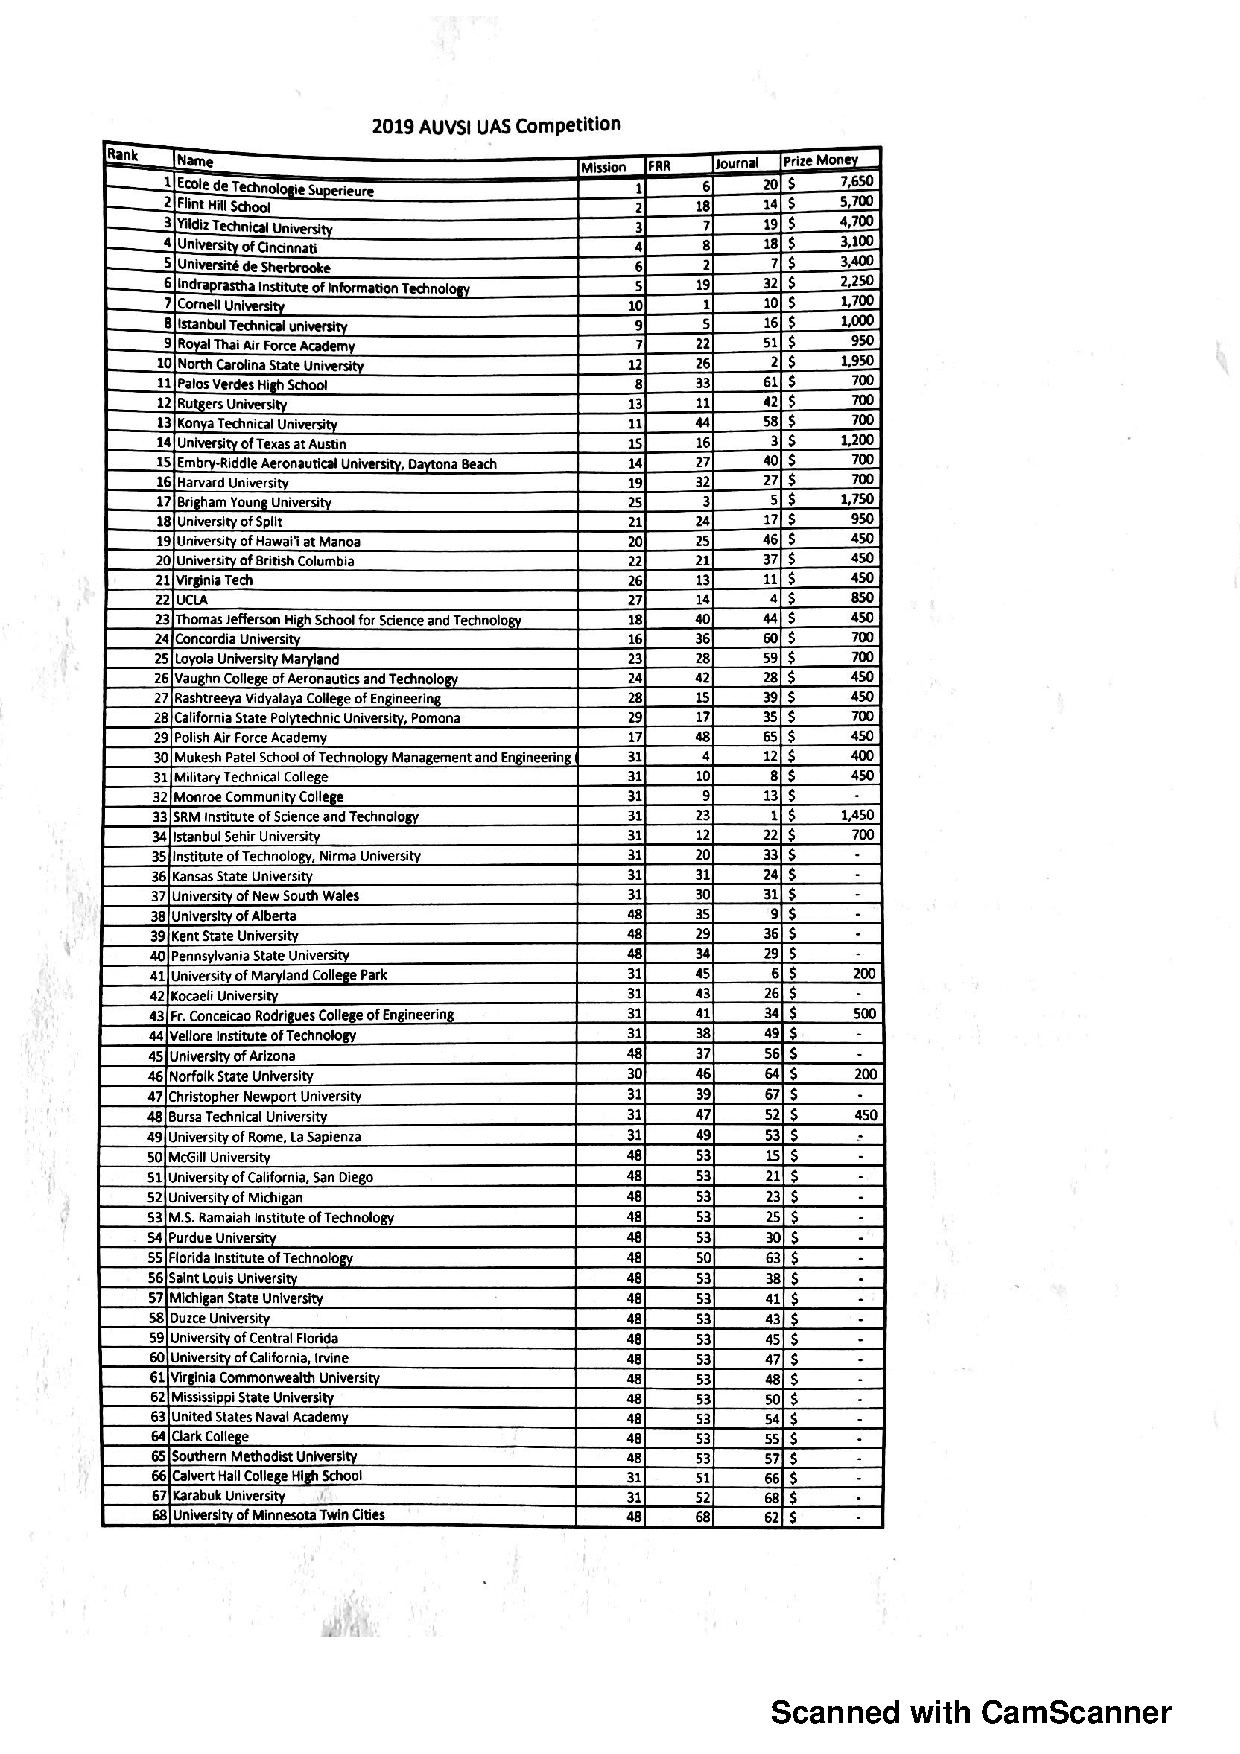
\includepdf[pages=-,  offset=75 -75]{./BYU-AUVSI-2019_Scores_and_Judges_Feedback.pdf}

\end{document}
